\documentclass[12pt,a4paper]{article}

% ─── Page Layout ───────────────────────────────────────────────────────────────
\usepackage[a4paper, margin=0.8in, headheight=14pt]{geometry}

% ─── Fonts (XeLaTeX) ───────────────────────────────────────────────────────────
\usepackage{fontspec}
\usepackage{unicode-math}
\setmainfont{TeX Gyre Pagella}
\setmonofont[Scale=0.88]{TeX Gyre Cursor}
\setmathfont{Latin Modern Math}

% ─── Packages ──────────────────────────────────────────────────────────────────
\usepackage{xcolor}
\usepackage{colortbl}
\usepackage{titlesec}
\usepackage{enumitem}
\usepackage{tabularx}
\usepackage{booktabs}
\usepackage{array}
\usepackage{amsmath}
\usepackage{tikz}
\usetikzlibrary{shapes.geometric, arrows.meta, positioning, calc, fit, decorations.pathreplacing, decorations.pathmorphing}
\usepackage{tcolorbox}
\tcbuselibrary{skins, breakable}
\usepackage{hyperref}
\usepackage{fancyhdr}
\usepackage{graphicx}
\usepackage{microtype}
\hyphenpenalty=10000
\exhyphenpenalty=10000
\sloppy
\usepackage{caption}
\usepackage{setspace}
\usepackage{multirow}
\usepackage{tocloft}

% ─── Q&A helper ────────────────────────────────────────────────────────────────
\newcommand{\Q}[1]{\textbf{#1}\par\noindent\ignorespaces}

% ─── Colour Palette ────────────────────────────────────────────────────────────
\definecolor{myred}{RGB}{196,30,58}
\definecolor{mydark}{RGB}{30,30,50}
\definecolor{mygreen}{RGB}{14,120,80}
\definecolor{myteal}{RGB}{0,130,140}
\definecolor{myamber}{RGB}{180,100,0}
\definecolor{mypurple}{RGB}{100,30,160}
\definecolor{mygray}{RGB}{246,247,249}
\definecolor{mgframe}{RGB}{180,185,200}
\definecolor{watermark}{RGB}{145,150,170}
\definecolor{hdrred}{RGB}{250,232,235}
\definecolor{hdrgreen}{RGB}{220,244,233}
\definecolor{hdrteal}{RGB}{220,242,244}
\definecolor{hdramber}{RGB}{253,242,215}
\definecolor{hdrpurple}{RGB}{238,228,255}
\definecolor{hdrgray}{RGB}{238,240,245}
\definecolor{rowalt}{RGB}{250,251,253}

% ─── Section Formatting ────────────────────────────────────────────────────────
\titleformat{\section}
  {\large\bfseries\color{myred}}{\thesection.}{0.5em}{}
  [\vspace{1pt}{\color{myred}\rule{\linewidth}{0.8pt}}]
\titleformat{\subsection}
  {\normalsize\bfseries\color{myteal}}{\thesubsection}{0.5em}{}
\titlespacing*{\section}{0pt}{18pt}{7pt}
\titlespacing*{\subsection}{0pt}{11pt}{4pt}

% ─── Paragraph ─────────────────────────────────────────────────────────────────
\setlength{\parindent}{0pt}
\setlength{\parskip}{4pt}

% ─── TOC Styling ───────────────────────────────────────────────────────────────
\renewcommand{\cfttoctitlefont}{\large\bfseries\color{myred}}
\renewcommand{\cftaftertoctitle}{\par\noindent{\color{myred}\rule{\linewidth}{0.8pt}}}
\setlength{\cftbeforetoctitleskip}{0pt}
\setlength{\cftaftertoctitleskip}{6pt}
\renewcommand{\cftsecfont}{\normalsize\bfseries\color{mydark}}
\renewcommand{\cftsecpagefont}{\normalsize\bfseries\color{mydark}}
\renewcommand{\cftsecleader}{\cftdotfill{\cftdotsep}}
\setlength{\cftbeforesecskip}{7pt}
\renewcommand{\cftsubsecfont}{\small\color{mydark}}
\renewcommand{\cftsubsecpagefont}{\small\color{mydark}}
\setlength{\cftbeforesubsecskip}{3pt}
\setlength{\cftsubsecindent}{1.4em}

% ─── Table helpers ─────────────────────────────────────────────────────────────
\renewcommand{\arraystretch}{1.45}
\setlength{\tabcolsep}{6pt}
\arrayrulecolor{mydark}
\newcolumntype{B}[1]{>{\small\bfseries\raggedright\arraybackslash}m{#1}}
\newcolumntype{C}[1]{>{\centering\arraybackslash}m{#1}}
\newcolumntype{Y}{>{\small\raggedright\arraybackslash}X}
\renewcommand{\tabularxcolumn}[1]{m{#1}}

% ─── Header / Footer ───────────────────────────────────────────────────────────
\pagestyle{fancy}
\fancyhf{}
\fancyhead[L]{\small\color{myred}\textbf{PE-EC703C}\;\color{mydark}--- Wavelet Transforms}
\fancyhead[R]{\small\color{myteal}\textbf{Module 4 Notes}}
\fancyfoot[C]{\small\color{mydark}\thepage}
\fancyfoot[R]{\small\color{watermark}\textit{\copyright\ Biraj Sarkar}}
\renewcommand{\headrulewidth}{0.5pt}
\renewcommand{\footrulewidth}{0.3pt}

% ─── Hyperref ──────────────────────────────────────────────────────────────────
\hypersetup{
  colorlinks=true, linkcolor=myteal, urlcolor=myteal,
  pdfauthor={Biraj Sarkar},
  pdftitle={PE-EC703C --- Module 4 Notes}
}

% ─── tcolorbox styles ──────────────────────────────────────────────────────────
\tcbset{
  tikzbox/.style={
    colback=mygray, colframe=mgframe, boxrule=0.6pt, arc=4pt,
    left=8pt, right=8pt, top=6pt, bottom=6pt,
    colbacktitle=mgframe, coltitle=mydark,
    fonttitle=\small\bfseries
  },
  defbox/.style={
    colback=hdrgreen, colframe=mygreen, boxrule=0.8pt, arc=4pt,
    left=9pt, right=9pt, top=6pt, bottom=6pt,
    colbacktitle=mygreen, coltitle=white,
    fonttitle=\small\bfseries
  },
  formulabox/.style={
    colback=hdrteal, colframe=myteal, boxrule=0.8pt, arc=4pt,
    left=9pt, right=9pt, top=7pt, bottom=7pt,
    colbacktitle=myteal, coltitle=white,
    fonttitle=\small\bfseries
  },
  examplebox/.style={
    colback=hdramber, colframe=myamber, boxrule=0.8pt, arc=4pt,
    left=9pt, right=9pt, top=6pt, bottom=6pt,
    colbacktitle=myamber, coltitle=white,
    fonttitle=\small\bfseries
  },
  masonbox/.style={
    colback=hdrpurple, colframe=mypurple, boxrule=0.8pt, arc=4pt,
    left=9pt, right=9pt, top=6pt, bottom=6pt,
    colbacktitle=mypurple, coltitle=white,
    fonttitle=\small\bfseries
  },
  exambox/.style={
    colback=hdrpurple, colframe=mypurple, boxrule=1pt, arc=5pt,
    left=10pt, right=10pt, top=8pt, bottom=8pt,
    colbacktitle=mypurple, coltitle=white,
    fonttitle=\bfseries,
    breakable, title after break={\textbf{Frequently Asked / Viva Questions (contd.)}}}
}
\tcbset{breakable}

% ─── TikZ styles ───────────────────────────────────────────────────────────────
\tikzset{
  block/.style={rectangle, draw=myteal, fill=hdrteal,
    text width=2.2cm, align=center, minimum height=0.9cm,
    font=\small, rounded corners=3pt, line width=0.7pt},
  redblock/.style={rectangle, draw=myred, fill=hdrred,
    text width=2.2cm, align=center, minimum height=0.9cm,
    font=\small, rounded corners=3pt, line width=0.7pt},
  arrow/.style={-Stealth, thick, color=mydark},
  redarrow/.style={-Stealth, thick, color=myred},
  line/.style={thick, color=mydark}
}

% ═══════════════════════════════════════════════════════════════════════════════
\begin{document}
% ═══════════════════════════════════════════════════════════════════════════════

\begin{center}
  {\LARGE\bfseries\color{myred} PE-EC703C --- Wavelet Transforms}\\[5pt]
  {\normalsize\color{mydark} Semester VII \quad$\bullet$\quad 3L:0T:0P \quad$\bullet$\quad 3 Credits}\\[3pt]
  {\normalsize\color{myteal}\textbf{Module 4 Exam Notes: Bi-orthogonal \& Multi-dimensional Wavelets}}\\[3pt]
  {\small\color{mydark} CGEC \;$|$\; B.Tech ECE (2023--27) \;$|$\; \textit{Biraj Sarkar}}
\end{center}
\vspace{2pt}
\noindent{\color{myred}\rule{\linewidth}{1.5pt}}
\vspace{2pt}

\hypersetup{linkcolor=mydark}
\tableofcontents
\hypersetup{linkcolor=myteal}
\newpage

% ===============================================================================
\section{Bi-orthogonal Wavelets}
% ===============================================================================

Orthonormal wavelets (like the Daubechies family) cannot be symmetric (except for the Haar wavelet). In image processing, asymmetry introduces phase distortion, which is highly visible. To achieve both \textbf{compact support}, \textbf{orthogonality}, and \textbf{symmetry} (linear phase), we relax the self-orthogonality requirement and use \textbf{Bi-orthogonal Wavelets}.

\subsection{Dual Scaling and Wavelet Functions}
A bi-orthogonal wavelet system uses two scaling functions ($\phi$, $\tilde{\phi}$) and two wavelet functions ($\psi$, $\tilde{\psi}$):
\begin{itemize}[leftmargin=*, itemsep=3.5pt]
  \item $\phi(t)$ and $\psi(t)$ are used for \textbf{decomposition (Analysis)}.
  \item $\tilde{\phi}(t)$ and $\tilde{\psi}(t)$ are used for \textbf{reconstruction (Synthesis)}.
\end{itemize}

They satisfy the \textbf{cross-orthogonality (bi-orthogonality)} conditions:
$$\langle \phi(t), \tilde{\phi}(t-k) \rangle = \delta[k], \quad \langle \psi(t), \tilde{\psi}(t-k) \rangle = \delta[k]$$
$$\langle \phi(t), \tilde{\psi}(t-k) \rangle = 0, \quad \langle \psi(t), \tilde{\phi}(t-k) \rangle = 0$$
where $\delta[k]$ is the Kronecker delta.

\subsection{Bi-orthogonal Filter Perfect Reconstruction Conditions}
In the $Z$-domain, the analysis filters ($H_0, H_1$) and synthesis filters ($\tilde{H}_0, \tilde{H}_1$) must satisfy:
$$H_0(z)\tilde{H}_0(z^{-1}) + H_1(z)\tilde{H}_1(z^{-1}) = 2$$
$$H_0(-z)\tilde{H}_0(z^{-1}) + H_1(-z)\tilde{H}_1(z^{-1}) = 0$$
These conditions allow the filters to have symmetric coefficients (linear phase response).

\subsection{Popular Bi-orthogonal Wavelets: CDF 9/7 and 5/3}
\begin{itemize}[leftmargin=*, itemsep=4.5pt]
  \item \textbf{CDF 9/7 Wavelet:} The Cohen-Daubechies-Feauveau 9/7 wavelet has 9 low-pass analysis coefficients and 7 low-pass synthesis coefficients. It has high smoothness and vanishing moments, making it the industry standard for lossy image compression (\textbf{JPEG 2000} standard).
  \item \textbf{CDF 5/3 Wavelet:} Has 5 analysis coefficients and 3 synthesis coefficients. It utilizes integer-to-integer mappings, enabling \textbf{lossless} (reversible) image compression.
\end{itemize}

% ===============================================================================
\section{Two-Dimensional Wavelets}
% ===============================================================================

To analyze 2D signals (images), we extend the 1D MRA to $L^2(\mathbb{R}^2)$.

\subsection{Separable 2D Wavelet Decomposition}
A separable 2D wavelet transform uses the tensor product of 1D scaling and wavelet functions:
\begin{enumerate}[leftmargin=*, itemsep=4.5pt]
  \item \textbf{2D Scaling Function (Approximation):}
        $$\Phi(x,y) = \phi(x)\phi(y) \quad \implies \text{LL Subband (Low-Low)} = \text{Coarse Approximation}$$
  \item \textbf{2D Wavelet Functions (Details):}
        \begin{itemize}[leftmargin=*, itemsep=3pt, topsep=3pt]
          \item $\Psi^H(x,y) = \phi(x)\psi(y) \quad \implies \text{HL Subband (Low-High)} = \text{Horizontal Details}$
          \item $\Psi^V(x,y) = \psi(x)\phi(y) \quad \implies \text{LH Subband (High-Low)} = \text{Vertical Details}$
          \item $\Psi^D(x,y) = \psi(x)\psi(y) \quad \implies \text{HH Subband (High-High)} = \text{Diagonal Details}$
        \end{itemize}
\end{enumerate}

\newpage
\begin{tcolorbox}[tikzbox, title={2D DWT Separable Quadrant Subbands (3-Level Grid)}]
\centering
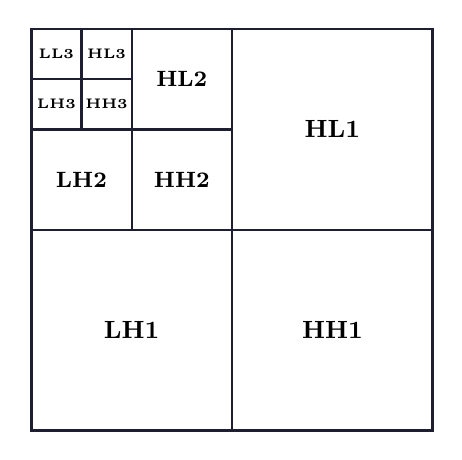
\begin{tikzpicture}[scale=0.85]
  % Boundary Box
  \draw[draw=mydark, line width=1pt] (0,0) rectangle (6,6);
  
  % Level 1 division
  \draw[line] (3,0) -- (3,6);
  \draw[line] (0,3) -- (6,3);
  \node[font=\small\bfseries] at (4.5, 4.5) {HL1};
  \node[font=\small\bfseries] at (1.5, 1.5) {LH1};
  \node[font=\small\bfseries] at (4.5, 1.5) {HH1};
  
  % Level 2 division
  \draw[line] (1.5,3) -- (1.5,6);
  \draw[line] (0,4.5) -- (3,4.5);
  \node[font=\footnotesize\bfseries] at (2.25, 5.25) {HL2};
  \node[font=\footnotesize\bfseries] at (0.75, 3.75) {LH2};
  \node[font=\footnotesize\bfseries] at (2.25, 3.75) {HH2};
  
  % Level 3 division
  \draw[line] (0.75,4.5) -- (0.75,6);
  \draw[line] (0,5.25) -- (1.5,5.25);
  \node[font=\tiny\bfseries] at (0.375, 5.625) {LL3};
  \node[font=\tiny\bfseries] at (1.125, 5.625) {HL3};
  \node[font=\tiny\bfseries] at (0.375, 4.875) {LH3};
  \node[font=\tiny\bfseries] at (1.125, 4.875) {HH3};
\end{tikzpicture}
\end{tcolorbox}

\subsection{Non-Separable Multi-dimensional Wavelets}
Separable transforms prioritize horizontal and vertical directions. \textbf{Non-separable 2D wavelets} use non-diagonal dilation matrices (like \textbf{Quincunx sampling}), splitting the frequency spectrum diagonally. This offers isotropic directional resolution and is less computationally redundant.

% ===============================================================================
\section{Wavelet Packets}
% ===============================================================================

\begin{tcolorbox}[defbox, title={\textbf{Definition of Wavelet Packets}}]
In a standard DWT, only the low-frequency approximation coefficients ($a_j$) are decomposed at each step. \textbf{Wavelet Packets (WP)} generalize this by recursively decomposing \textbf{both} approximation ($a_j$) and detail ($d_j$) coefficients, forming a \textbf{full binary tree} representation of the signal.
\end{tcolorbox}

\begin{tcolorbox}[tikzbox, title={Wavelet Packet (WP) vs. Standard DWT Trees}]
\centering
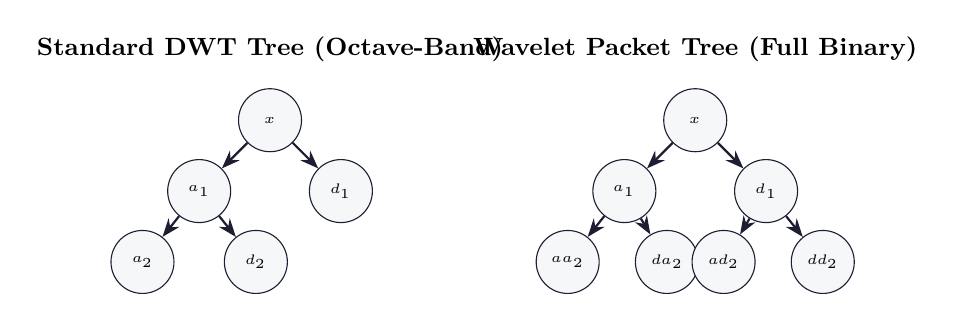
\begin{tikzpicture}[scale=0.9,
  node/.style={circle, draw=mydark, fill=mygray, minimum size=0.8cm, font=\tiny\bfseries}]
  
  % Standard DWT Tree
  \node at (1.5,2.5) {\small\bfseries Standard DWT Tree (Octave-Band)};
  \node[node] (s0) at (1.5,1.5) {$x$};
  \node[node] (sa1) at (0.5,0.5) {$a_1$};
  \node[node] (sd1) at (2.5,0.5) {$d_1$};
  \node[node] (sa2) at (-0.3,-0.5) {$a_2$};
  \node[node] (sd2) at (1.3,-0.5) {$d_2$};
  \draw[arrow] (s0) -- (sa1);
  \draw[arrow] (s0) -- (sd1);
  \draw[arrow] (sa1) -- (sa2);
  \draw[arrow] (sa1) -- (sd2);

  % Wavelet Packet Tree
  \node at (7.5,2.5) {\small\bfseries Wavelet Packet Tree (Full Binary)};
  \node[node] (w0) at (7.5,1.5) {$x$};
  \node[node] (wa1) at (6.5,0.5) {$a_1$};
  \node[node] (wd1) at (8.5,0.5) {$d_1$};
  \node[node] (wa2) at (5.7,-0.5) {$aa_2$};
  \node[node] (wad2) at (7.1,-0.5) {$da_2$};
  \node[node] (wda2) at (7.9,-0.5) {$ad_2$};
  \node[node] (wd2) at (9.3,-0.5) {$dd_2$};
  \draw[arrow] (w0) -- (wa1);
  \draw[arrow] (w0) -- (wd1);
  \draw[arrow] (wa1) -- (wa2);
  \draw[arrow] (wa1) -- (wad2);
  \draw[arrow] (wd1) -- (wda2);
  \draw[arrow] (wd1) -- (wd2);
\end{tikzpicture}
\tcbset{after={\color{black}}}
\end{tcolorbox}

\textbf{Advantages of Wavelet Packets:}
\begin{itemize}[leftmargin=*, itemsep=4.5pt]
  \item \textbf{Rich Spectral Breakdown:} Yields $2^J$ subbands at level $J$, dividing the frequency spectrum uniformly (equal-width subbands).
  \item \textbf{Best Basis Selection:} Using entropy metrics (like \textbf{Shannon entropy}), the algorithm selects the optimal path through the tree to maximize sparsity, matching the signal's specific frequency patterns.
\end{itemize}

\newpage
% ===============================================================================
\begin{center}
  {\large\bfseries\color{myred} Quick Revision --- Module 4}\\[3pt]
  {\small\color{mydark} Bi-orthogonal \& Multi-dimensional Wavelets $|$ PE-EC703C}
\end{center}
\noindent{\color{myred}\rule{\linewidth}{1.2pt}}
\vspace{4pt}
% ===============================================================================

\begin{tcolorbox}[formulabox, title={\textbf{Key Equations}}]
\renewcommand{\arraystretch}{1.35}
\begin{tabularx}{\linewidth}{B{5.0cm} X}
Bi-orthogonality Rel. & $\langle \phi(t), \tilde{\phi}(t-k) \rangle = \delta[k], \quad \langle \psi(t), \tilde{\psi}(t-k) \rangle = \delta[k]$ \\[4pt]
PR filter condition & $H_0(z)\tilde{H}_0(z^{-1}) + H_1(z)\tilde{H}_1(z^{-1}) = 2$ \\[4pt]
2D Approximation (LL) & $\Phi(x,y) = \phi(x)\phi(y)$ \\[4pt]
2D Horiz. Wavelet (HL) & $\Psi^H(x,y) = \phi(x)\psi(y)$ \\[4pt]
2D Vert. Wavelet (LH) & $\Psi^V(x,y) = \psi(x)\phi(y)$ \\[4pt]
2D Diag. Wavelet (HH) & $\Psi^D(x,y) = \psi(x)\psi(y)$
\end{tabularx}
\tcbset{after={\color{black}}}
\end{tcolorbox}

\begin{tcolorbox}[defbox, title={\textbf{One-Line Definitions}}]
\begin{itemize}[leftmargin=*, itemsep=3.5pt]
  \item \textbf{Bi-orthogonal Wavelet:} A wavelet system utilizing dual, cross-orthogonal scaling and wavelet bases for decomposition and reconstruction.
  \item \textbf{Linear Phase:} Filter characteristic indicating constant group delay, preventing signal phase distortion.
  \item \textbf{CDF 9/7 Wavelet:} A symmetric biorthogonal filter family used for lossy image compression in JPEG 2000.
  \item \textbf{Separable 2D DWT:} 2D transform implemented by running 1D transforms along rows and columns sequentially.
  \item \textbf{Non-separable Wavelet:} A 2D wavelet transform using multi-directional sampling grids (e.g. Quincunx).
  \item \textbf{Wavelet Packet:} Decompositions where both low-pass and high-pass branches are recursively filtered.
\end{itemize}
\end{tcolorbox}

\begin{tcolorbox}[exambox, title={\textbf{Frequently Asked / Viva Questions}}]
\begin{enumerate}[topsep=0pt, label=\textbf{Q\arabic*.}, itemsep=5pt]
  \item \Q{Why do we need bi-orthogonal wavelets in image processing?}
        In image processing, phase distortion must be avoided. Orthonormal wavelets (except Haar) cannot be symmetric (which is required for linear phase). Bi-orthogonal wavelets decouple decomposition and reconstruction, allowing filters to be symmetric and linear-phase while remaining compactly supported.

  \item \Q{What is the difference between CDF 9/7 and CDF 5/3 filters in JPEG 2000?}
        The CDF 9/7 filter has 9 analysis and 7 synthesis coefficients. It is used for lossy compression because it has high vanishing moments and excellent energy compaction. The CDF 5/3 filter has 5 analysis and 3 synthesis coefficients, uses integer coefficients, and is used for lossless compression.

  \item \Q{Explain separable 2D wavelet decomposition.}
        A separable 2D wavelet transform is computed by applying the 1D DWT horizontally along each row of the image, followed by applying the 1D DWT vertically along each column. This decomposes the image into four subbands: LL (approximation), LH (vertical details), HL (horizontal details), and HH (diagonal details).

  \item \Q{What is Quincunx sampling in multi-dimensional wavelets?}
        Quincunx sampling is a non-separable 2D downsampling scheme. It reduces the sampling grid by a factor of 2 in a diagonal checkerboard pattern. It provides isotropic frequency responses, avoiding the horizontal/vertical directional bias of separable transforms.

  \item \Q{How do Wavelet Packets differ from standard DWT?}
        A standard DWT only decomposes the approximation subband ($a_j$) at each level. A Wavelet Packet transform recursively decomposes both the approximation ($a_j$) and detail ($d_j$) subbands, generating a full binary tree. This provides higher spectral resolution at high frequencies.

  \item \Q{What is "best basis selection" in Wavelet Packets?}
        Since Wavelet Packets generate a redundant binary tree, we must select the most efficient subbands. The best basis algorithm evaluates the entropy (e.g. Shannon entropy) of each node and prunes the tree to minimize representation cost.
\end{enumerate}
\end{tcolorbox}

\begin{tcolorbox}[tikzbox, title={\textbf{Summary Comparison: DWT vs. Wavelet Packets}}]
\par\noindent
{\renewcommand{\arraystretch}{1.4}%
\begin{tabularx}{\linewidth}{|B{3.2cm}|Y|Y|}
\hline
\textbf{Feature} & \textbf{Standard DWT} & \textbf{Wavelet Packets (WP)} \\
\hline
\textbf{Decomposition Tree} & Octave-band (unbalanced tree). & Full binary tree (symmetrical). \\
\hline
\textbf{Subbands at Level $J$} & $3J+1$ subbands. & $2^J$ subbands. \\
\hline
\textbf{Frequency Resolution} & Logarithmic (narrow at low frequencies). & Uniform (equal bandwidth bands). \\
\hline
\textbf{Adaptivity} & Rigid (fixed octaves). & Highly adaptive (best basis selection). \\
\hline
\textbf{Sparsity for Curves} & Poor (requires many coefficients). & Poor (struggles with curved features). \\
\hline
\end{tabularx}}
\end{tcolorbox}

\end{document}
